\chapter[Metodología de Trabajo]{Metodología de Trabajo}
\label{cp:methodology}

\parindent0pt

Para la consecución de los objetivos propuestos en este trabajo final, se ha definido una metodología de trabajo que permite planificar y gestionar las diferentes tareas y recursos del proyecto de manera ordenada. Por ello, en este capítulo se presentan los diferentes pasos que se ejecutaron para llegar a cumplir estos objetivos. 

Primeramente, se hablará sobre la planificación del trabajo, haciendo hincapié en las actividades necesarias para llevar a cabo el proyecto de forma ordenada y efectiva (Sección \ref{sec:work-plan}). Posteriormente, se describirá el Modelo en V, que es la metodología de desarrollo de software seleccionada como marco de referencia para la organización de las actividades de desarrollo del prototipo tecnológico. Se describirán las etapas del proceso de desarrollo, detallando las actividades y resultados esperados en cada una de ellas a partir de la metodología seleccionada. Finalmente, se profundizará en la gestión del proyecto, haciendo hincapié en las herramientas y prácticas seleccionadas para asegurar una gestión eficiente a lo largo de todas las fases del proceso de desarrollo del prototipo.

\section{Planificación del Trabajo}
\label{sec:work-plan}

Definir un plan de trabajo, previo al desarrollo del prototipo tecnológico, es una buena práctica que permite establecer una hoja de ruta concisa que sirve de guía orientativa a lo largo de todo el proceso. El plan de trabajo define los objetivos y actividades necesarios para llevar a cabo un proyecto eficazmente. Para este trabajo en particular, se definió un plan que comprende las actividades necesarias para poder desarrollar un prototipo tecnológico basado en blockchain, orientado a la trazabilidad y valorización del vidrio, con el objetivo de contribuir a la economía circular en la región. Este plan sirve de guía para la ejecución de las actividades y la toma de decisiones a lo largo del proyecto, pero es flexible y puede adaptarse a cambios y nuevas necesidades que puedan surgir durante el desarrollo del trabajo. En la Figura \ref{fig:activities-plan} se ilustran las actividades que conforman el plan de trabajo junto con su duración estimada y secuencialidad. A continuación se detalla el alcance y los objetivos de cada actividad.

\begin{figure}[!htb]
    \centering
    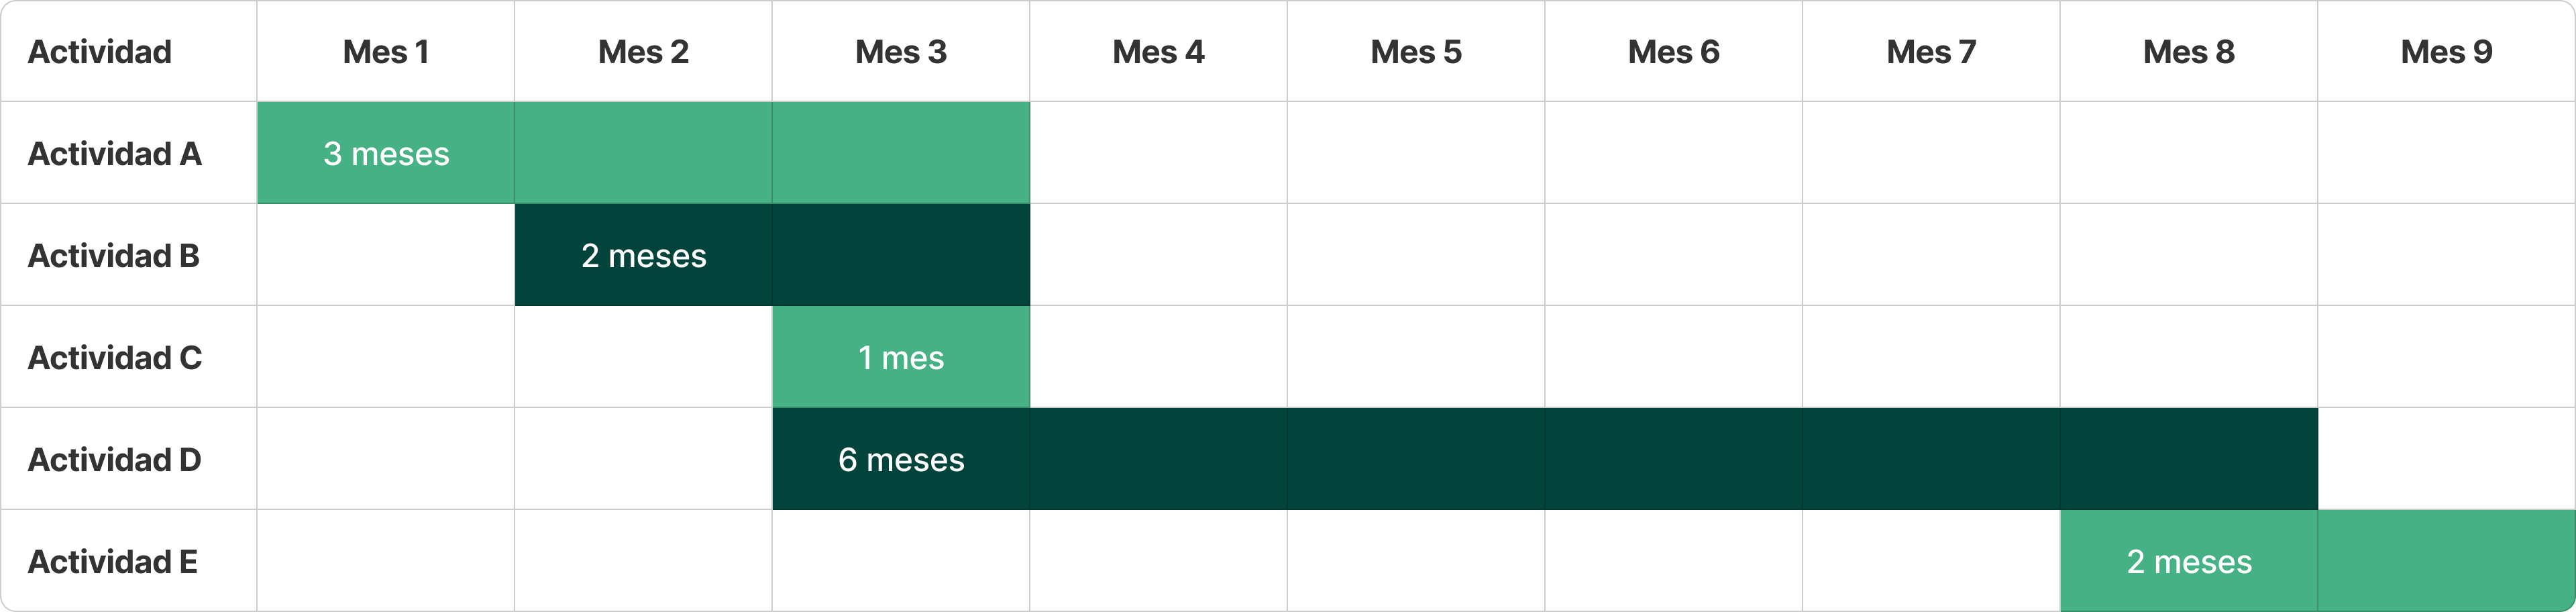
\includegraphics[width=\textwidth]{Figures/activities-plan.png}
    \caption{Organización de las actividades del plan de trabajo}
    \label{fig:activities-plan}
\end{figure}

\begin{itemize}
	\item \textbf{Actividad A}: completar la formación en blockchain y las tecnologías y plataformas relacionadas. Los resultados de esta formación se aplican posteriormente en las etapas de diseño de solución e implementación del prototipo tecnológico (comprendidas en la Actividad D).
	\item \textbf{Actividad B}: realizar un estudio pormenorizado del estado actual del arte en todo lo relacionado con blockchain en el campo del reciclado. En particular, la búsqueda se orienta al reciclado de vidrio. Se analizan trabajos de la literatura, así como aplicaciones blockchain orientadas al reciclaje y la cadena de suministro. Los resultados de este estudio se encuentran documentados en el Capítulo \ref{cp:theoretical-framework}: Marco Teórico y en los Apéndices \ref{cp:verallia-interview}: Entrevista a Verallia y \ref{cp:europe-trip}: Viaje de Investigación.
	\item \textbf{Actividad C}: definir los procesos de desarrollo del prototipo, haciendo hincapié en la aplicación de los fundamentos de la \gls{ingenieriadesoftware} y planificar de forma concisa y clara. En la Sección \ref{sec:software-method} se describe la metodología elegida para el proceso de desarrollo del prototipo tecnológico.
	\item \textbf{Actividad D}: desarrollar la aplicación prototipo. Esta actividad comprende las diferentes etapas del proceso de desarrollo de \gls{software}, desde el análisis de requerimientos, diseño, implementación, validación del prototipo y despliegue. Todos estos pasos se deben ejecutar siguiendo la metodología específica elegida para este trabajo durante la Actividad C, teniendo en cuenta las características particulares del modelo de proceso elegido, con el fin de llevar a cabo el objetivo general de este trabajo.
	\item \textbf{Actividad E}: documentar en una memoria el proceso ejecutado y los resultados del trabajo realizado.
\end{itemize}

La consecución de estas actividades requiere un marco metodológico que permita gestionar el desarrollo del prototipo de manera eficiente. En la siguiente sección, se detallará la metodología de desarrollo de software elegida para este proyecto y se justificarán los motivos de su selección.

% TODO: y esto? Lo mato o lo dejo en algún lado?

% \subsection{Delimitación del Alcance}
% El presente trabajo se centra en la tecnología blockchain como eje principal debido a su naturaleza disruptiva y su potencial para transformar la trazabilidad y la gestión de datos. La elección de la aplicación orientada a la economía circular se justifica por la relevancia actual de este área de impacto y la necesidad de soluciones sostenibles. Particularmente, el dominio se delimita al vidrio, siguiendo la recomendación de diversas investigaciones que sugieren que la especialización en un material particular permite obtener mejores resultados en usabilidad y tasas de reciclaje. Esto se debe a la posibilidad de diseñar sistemas a medida de los procesos productivos y de reciclaje del material elegido. El vidrio en particular es seleccionado como material reciclable para desarrollar este trabajo por sus características de alta reciclabilidad y su significativo impacto regional en Mendoza (provincia vitivinícola) cuya principal industria productiva, el vino, depende en gran medida de los envases de vidrio. La localización en Mendoza se debe a que este trabajo se desarrolla en la Universidad Nacional de Cuyo (UNCUYO), con sede principal en esta provincia.

\section{Metodología de Desarrollo}
\label{sec:software-method}

Para desarrollar un \gls{software} de calidad que cumpla con los objetivos planteados, es necesario seguir una metodología de desarrollo de software que asegure que se sigan buenas prácticas de \gls{ingenieriadesoftware} para poder entregar un producto funcional, estable, documentado y mantenible dentro de los plazos propuestos. Existen diversas metodologías de desarrollo de software que permiten planificar y ordenar el proceso de desarrollo de software para alcanzar los objetivos del proyecto haciendo un uso eficiente de los recursos disponibles. Cada metodología tiene sus propias características, ventajas y desventajas, y la elección de una metodología apropiada depende de las necesidades específicas del proyecto, tales como el alcance del prototipo, la frecuencia de entrega de resultados, la probabilidad de cambios en los requerimientos durante el desarrollo y la estructura del equipo de trabajo.

Las metodologías de desarrollo de software pueden clasificarse en dos grandes categorías: los modelos prescriptivos o tradicionales, que ofrecen una estructura y un orden definidos para maximizar la previsibilidad y la eficiencia en entornos con requerimientos estables, y los modelos evolutivos o ágiles, que se adaptan mejor a las realidades dinámicas del desarrollo de software moderno al permitir la iteración continua y la flexibilidad frente a los cambios \cite{pressman2010ingenieria}. Cada metodología propone una serie de etapas y prácticas que guían el proceso de desarrollo, como pueden ser la definición de requerimientos, el diseño, la implementación, las pruebas, la documentación, el despliegue y el mantenimiento del software.

Particularmente, en este trabajo se debe elegir una metodología de desarrollo de software que sea apropiada para un equipo unipersonal, ya que el desarrollo del prototipo tecnológico es llevado a cabo por una única persona. A su vez, la metodología debe ser adecuada para proyectos con un alcance definido desde el comienzo y con requerimientos relativamente estables, ya que el objetivo del trabajo es desarrollar un prototipo tecnológico funcional que cumpla con los requerimientos planteados inicialmente. Por último, el proyecto tiene una duración limitada con una única entrega del proyecto completo al final, por lo que la metodología debe permitir una planificación clara y concisa para cumplir con los plazos establecidos, aunque debe ser lo suficientemente flexible para adaptarse a cambios menores que puedan surgir durante el desarrollo del prototipo. Teniendo en cuenta estos factores, se decidió adoptar una metodología híbrida para el desarrollo del prototipo que combina el \textit{Modelo en V} (tradicional) con la gestión de tareas de \textit{Kanban} (ágil). El Modelo en V aporta un enfoque estructurado para la planificación y documentación del proyecto, mientras que Kanban proporciona flexibilidad para la gestión de tareas y el seguimiento del flujo de trabajo diario en un entorno unipersonal.

El Modelo en V (Figura \ref{fig:model-v}) es una extensión del \textit{Modelo en Cascada} que empareja cada fase de desarrollo con una fase de prueba correspondiente \cite{pressman2010ingenieria}. Este modelo propone una estructura de etapas en forma de ``V'', de modo que a medida que el proyecto avanza hacia abajo en la primera mitad de la V, los requerimientos y componentes del sistema son detallados cada vez más hasta llegar a la codificación, de forma similar al funcionamiento del Modelo en Cascada, donde cada fase debe completarse en orden sin contemplar posibles errores o cambios. Una vez completada la codificación, el proceso asciende por el lado derecho de la V, donde cada etapa de definición anterior es validada a través de pruebas específicas. A diferencia del Modelo en Cascada, el Modelo en V plantea una verificación sistemática en cada etapa, con el fin de detectar y corregir errores de forma temprana y minimizar riesgos al final del proyecto. Este modelo es apropiado para proyectos que requieren altos estándares de calidad y donde los errores tempranos podrían tener consecuencias costosas o críticas. En el caso de un prototipo basado en \glspl{contratointeligente}, la inmutabilidad de los contratos desplegados en la blockchain hace que la detección temprana de errores sea crítica para garantizar la calidad y la fiabilidad del prototipo final, ya que una vez desplegados, los contratos no pueden ser modificados para resolver errores o vulnerabilidades de seguridad.

\begin{figure}[!tb]
	\centering
	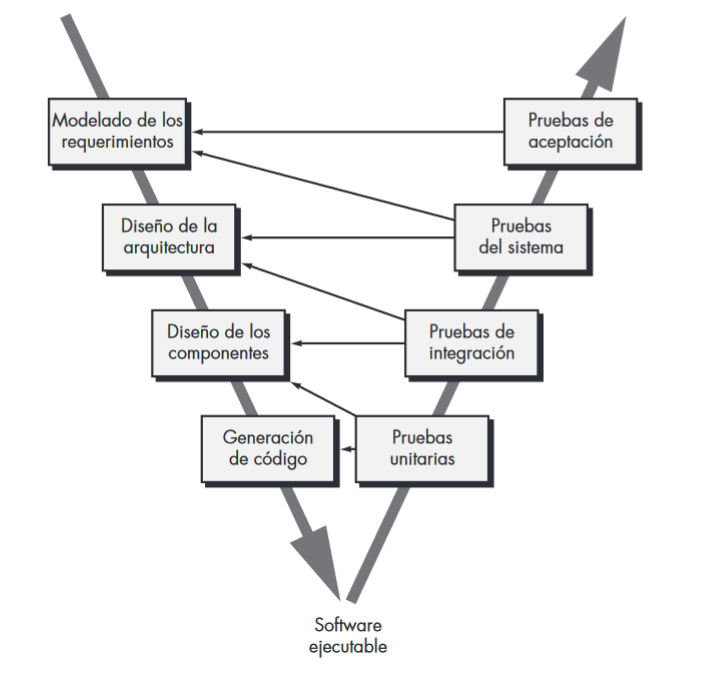
\includegraphics[width=0.6\textwidth]{Figures/model-v.png}
	\caption[Modelo en V]{Modelo en V. Fuente: \cite{pressman2010ingenieria}}
    \label{fig:model-v}
\end{figure}

Por otro lado, el método Kanban es un enfoque visual ágil para la gestión del flujo de trabajo, cuyo objetivo principal es optimizar la eficiencia al prevenir la sobrecarga de tareas y eliminar cuellos de botella \cite{alaidaros2021kanban}. Este método propone implementar un tablero visual dividido en columnas que representan las diferentes etapas del proceso de desarrollo, por donde se mueven las tareas o tarjetas. En la Figura \ref{fig:kanban-board} se muestra un ejemplo de un tablero Kanban para un proyecto en curso. Los principios de este modelo incluyen limitar el trabajo en curso, visualizar el flujo de tareas y medir su progreso para reconocer oportunidades de mejora. Kanban es una metodología ligera que se adapta bien a la situación de cualquier proyecto, es compatible con otras metodologías de trabajo y su implementación no requiere cambios estructurales en el proceso de trabajo. Sin embargo, su eficacia depende de una disciplina rigurosa y una comunicación constante del equipo para asegurar que el flujo visualizado en el tablero refleje la realidad actual del estado del proyecto. La naturaleza visual de Kanban facilita el seguimiento del progreso y permite una adaptación ágil a los cambios menores que puedan surgir en el día a día, sin comprometer la estructura general del proyecto \cite{alaidaros2021kanban}.

\begin{figure}[!tb]
    \centering
    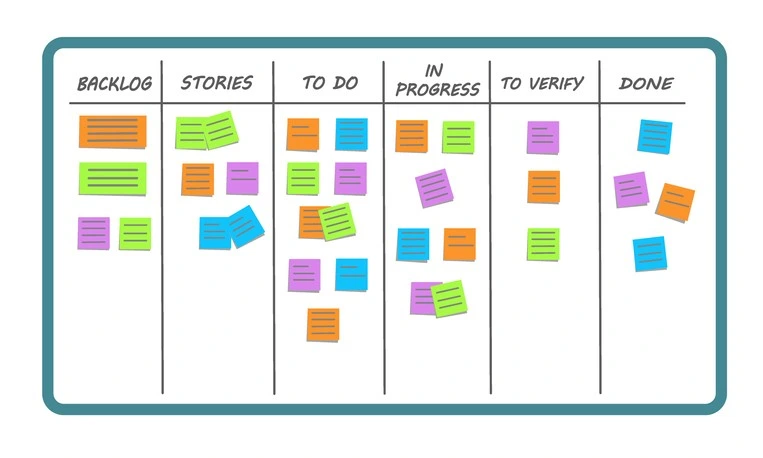
\includegraphics[width=0.9\textwidth]{Figures/model-kanban.png}
    \caption[Tablero Kanban]{Ejemplo de tablero Kanban}
    \label{fig:kanban-board}
\end{figure}

Por su parte, las metodologías ágiles presentan una flexibilidad que las hace adecuadas para proyectos con alta incertidumbre y cambios frecuentes en los requerimientos. Para este proyecto, se desestimó el uso de metodologías ágiles como \textit{Scrum}, ya que su estructura requiere la participación activa de un cliente para guiar reuniones recurrentes para la coordinación del equipo \cite{pressman2010ingenieria}, lo que no es aplicable a un proyecto académico individual. A su vez, el \textit{Modelo Espiral} es un enfoque iterativo robusto para gestionar riesgos y adaptarse a entornos inciertos \cite{pressman2010ingenieria}, pero tampoco se consideró apropiado para el alcance de este prototipo debido a la complejidad de su proceso evolutivo. En este caso, el proceso resultaría en una sobrecarga innecesaria para el alcance de este prototipo, dado que los requerimientos del trabajo están claramente definidos y la investigación preliminar ha minimizado la incertidumbre en el proceso.

En el contexto del desarrollo de un prototipo tecnológico basado en blockchain, la combinación del Modelo en V y Kanban representa la opción más estratégica. El Modelo en V proporciona la estructura necesaria para un proyecto con requerimientos estables y una necesidad crítica de alta calidad y fiabilidad. La validación rigurosa que propone este modelo, desde el diseño hasta las pruebas finales, asegura que se detecten y corrijan los errores de forma temprana. Por otro lado, Kanban ofrece flexibilidad operativa para gestionar las tareas del día a día de manera visual, lo que facilita el seguimiento del progreso del proyecto y la adaptación a cambios menores en la planificación.

La elección de esta metodología híbrida busca mantener un enfoque sistemático y estructurado, al mismo tiempo que se aprovecha la flexibilidad operativa en el manejo de tareas diarias. El siguiente apartado abordará en detalle cada etapa del proceso de desarrollo en el contexto del Modelo en V, desde el modelado de requerimientos hasta las pruebas, para llevar a cabo el desarrollo del prototipo tecnológico.

\subsection{Etapas del Proceso de Desarrollo}

Utilizando el Modelo en V como marco de referencia, el desarrollo del sistema se concibe como un proceso estructurado que se divide en dos grandes fases: la fase descendente, que se enfoca en la definición, el diseño y la implementación, y la fase ascendente, que se centra en la verificación y las pruebas. A continuación, se detallan las actividades y los resultados esperados de cada una de las etapas del proceso de desarrollo, siguiendo el modelo en V, aplicado al prototipo de trazabilidad del vidrio basado en blockchain. En la Figura \ref{fig:methodology-v-grouped} se muestran las etapas del proceso de desarrollo en V agrupadas en bloques temáticos, con el fin de ilustrar de manera más clara las interacciones y dependencias entre las diferentes fases de desarrollo de este trabajo.

\begin{figure}[!b]
	\centering
	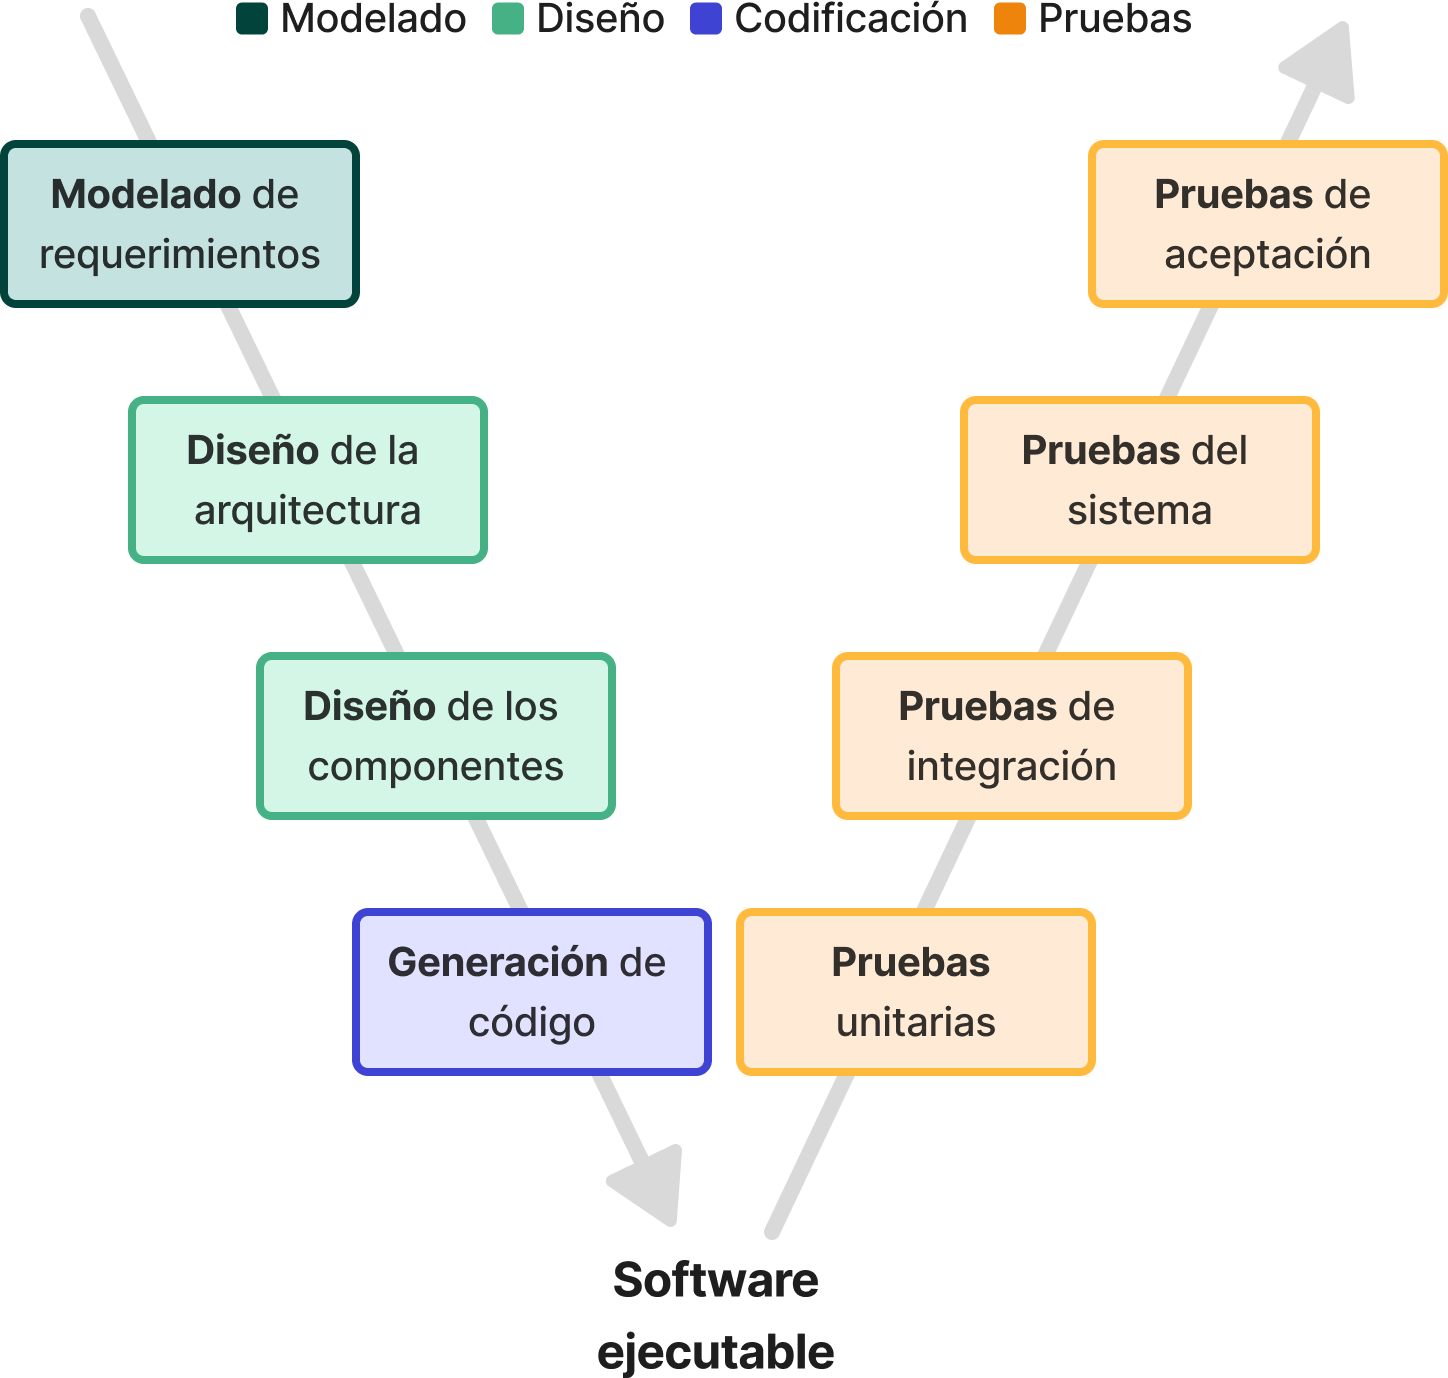
\includegraphics[width=0.6\textwidth]{Figures/model-v-grouped.png}
	\caption{Modelo en V agrupado por etapas}
    \label{fig:methodology-v-grouped}
\end{figure}


\textbf{Modelado de requerimientos:}
Es la primera fase del proceso, comprende la identificación y documentación detallada de los requerimientos funcionales y no funcionales del prototipo.
Los hallazgos se nutren directamente de la investigación realizada como parte de la Actividad B, comprendiendo la revisión del estado del arte en blockchain, gestión de residuos y trazabilidad, así como las entrevistas y las observaciones de programas de reciclaje existentes.
El objetivo en esta etapa es comprender las necesidades específicas del sistema de trazabilidad del vidrio para definir un conjunto exhaustivo de requerimientos que aseguren que el prototipo aborde los desafíos identificados en la cadena de producción de envases de vidrio en la región.
El resultado de esta fase es un documento de requerimientos funcionales y no funcionales que sirve como guía para las siguientes etapas del desarrollo.
La ejecución y resultados de esta fase se detallan en el Capítulo \ref{cp:modelling}.

\textbf{Diseño:}
El diseño del sistema se divide en dos etapas: diseño de arquitectura y diseño de componentes.
En la primera etapa, se define la arquitectura general del sistema, incluyendo la selección de tecnologías y plataformas a utilizar, así como la estructura de los módulos principales y la división de responsabilidades entre ellos.
En la segunda etapa, se realiza el diseño detallado de cada componente de los módulos del sistema, especificando las interfaces, protocolos de comunicación y estructuras de datos a utilizar.
El diseño en etapas y previo a la implementación tiene el objetivo de garantizar que el sistema sea escalable, mantenible y cumpla con los requerimientos definidos en la fase anterior.
El resultado es un conjunto de documentos de diseño que guían la implementación del prototipo. En el Capítulo \ref{cp:design} se presentan los detalles de la ejecución de estas dos fases de diseño del sistema.

\textbf{Generación de código:}
Durante la fase de generación de código o implementación, se lleva a cabo la codificación del prototipo, cada módulo y sus componentes en las tecnologías elegidas y especificaciones detalladas durante la etapa de diseño.
Esta etapa es gestionada con el apoyo de Kanban para la organización y seguimiento de las micro-tareas para mantener un flujo de trabajo ágil y adaptable a los cambios menores que puedan surgir durante el desarrollo.
El resultado de esta fase es un prototipo funcional que implementa los requerimientos y diseños definidos previamente.
En simultáneo con la generación de código se realiza la primera etapa de validación, que consiste en pruebas unitarias de cada componente desarrollado.
Estas pruebas aseguran que cada componente funcione correctamente de forma aislada y cumpla con los requerimientos funcionales especificados.
Al finalizar esta etapa, el software ejecutable está listo para ser desplegado en un entorno de pruebas. El despliegue del prototipo en un entorno de pruebas accesible públicamente (similar a un entorno productivo real) permite evaluar el comportamiento del sistema en condiciones reales y detectar posibles problemas antes de su uso final. A su vez, el entorno de pruebas es necesario para la realización de pruebas de integración y sistema en las etapas posteriores.
Los detalles de la implementación, las pruebas unitarias realizadas y el despliegue se describen en el Capítulo \ref{cp:implementation}.

\textbf{Pruebas:}
El proceso de pruebas se lleva a cabo en múltiples etapas.
Después de las pruebas unitarias, se realizan pruebas de integración automatizadas para verificar que los diferentes módulos del sistema interactúan correctamente entre sí a través de sus interfaces.
Estas pruebas aseguran que los datos fluyan adecuadamente dentro del sistema.
Posteriormente, se llevan a cabo pruebas de sistema para evaluar el comportamiento del prototipo en su conjunto para validar que el sistema cumple con los requerimientos funcionales y no funcionales definidos.
Las pruebas de sistema incluyen pruebas manuales para validar consistencia de datos en el sistema y corroborar que el prototipo cumple con los requerimientos funcionales, junto con pruebas automatizadas mediante código, que permiten verificar los requerimientos no funcionales como rendimiento y seguridad bajo condiciones simuladas.
Finalmente, se realizan pruebas de aceptación con un conjunto de usuarios voluntarios para validar que el prototipo cumple con los criterios de aceptación establecidos en la fase de modelado de requerimientos.
Los detalles de las pruebas realizadas en estas etapas de pruebas se presentan en el Capítulo \ref{cp:testing}.

\section{Gestión del Proyecto}

Para asegurar una gestión eficiente a lo largo de todas las fases del proceso de desarrollo es necesario implementar herramientas y prácticas de control de proyectos. La gestión del proyecto comprende la planificación, organización y supervisión de todas las actividades relacionadas con el desarrollo del prototipo, asegurando que se cumplan los plazos, se gestionen los recursos de manera efectiva y se mantenga la calidad del trabajo realizado.

Para la gestión de tareas diarias y el seguimiento del progreso del proyecto mediante Kanban, se decidió hacer uso de la herramienta Jira \footnote{\url{https://www.atlassian.com/es/software/jira}}. Este \gls{software} de gestión de proyectos de desarrollo de software provee una funcionalidad de tablero Kanban y permite gestionar el flujo de trabajo, asignar tareas a los miembros del equipo y realizar un seguimiento del progreso durante el desarrollo a través de una aplicación web con una interfaz intuitiva. 

A su vez, se determinó utilizar el software Git para el control de versiones del código fuente, una herramienta que permite un seguimiento detallado, seguro y ordenado de los cambios en el código. Git permite revertir cambios, comparar versiones y mantener un historial completo de modificaciones del código fuente, lo que permite programar de manera ordenada y segura en caso de problemas que puedan surgir durante el desarrollo. Junto con Git, se utiliza la plataforma GitHub \footnote{\url{https://github.com}}, que permite almacenar y gestionar repositorios de código en la nube, permitiendo el acceso remoto y público al código del proyecto. En el Apéndice \ref{cp:annex-content} se detallan los enlaces a los recursos adicionales relacionados con el proyecto, incluyendo la dirección del repositorio de código fuente en GitHub.

Por otro lado, es necesario definir la estrategia de documentación del proyecto de software previamente al inicio del desarrollo. La documentación forma parte del proceso de desarrollo de software y es un entregable en sí mismo, ya que proporciona una referencia clara y confiable sobre el diseño, la implementación y el uso del sistema para los desarrolladores actuales y futuros del proyecto. En este trabajo, se decidió adoptar una estrategia de documentación continua a lo largo de todas las etapas del proceso de desarrollo. Documentar cada fase del Modelo en V, desde la definición de requerimientos hasta las pruebas y el despliegue, asegura que toda la información relevante esté disponible para futuras referencias y facilita la comprensión del sistema por parte de otros desarrolladores o partes interesadas. En el caso del código fuente, se combinan dos enfoques: la documentación mediante comentarios en el código y la documentación externa, que comprende documentos separados dentro del repositorio de código fuente, que describen la arquitectura del sistema, instrucciones de instalación, guías de prueba y cualquier otra información relevante para entender y mantener el código del proyecto.

A partir de la selección de la metodología de desarrollo de software y la estrategia de gestión del proyecto, en los próximos capítulos se presentará el proceso de ejecución llevado a cabo en este trabajo para cada una de las etapas planteadas, incluyendo los resultados obtenidos en cada una.
En el Capítulo \ref{cp:modelling} se describirá el proceso de modelado de requerimientos, donde se explica cómo se obtuvieron los requerimientos funcionales y no funcionales, su priorización y la planificación del desarrollo.
En el Capítulo \ref{cp:design} se abordará el diseño del sistema, incluyendo la elección de tecnologías, diseño de arquitectura de software, modelado de la interfaz de usuario y definición de los módulos principales del prototipo.
Seguidamente, en el Capítulo \ref{cp:implementation} se detallará la implementación de cada módulo del sistema, integración de los módulos, pruebas unitarias realizadas y despliegue del prototipo en un entorno de pruebas similar a un entorno productivo.
En el Capítulo \ref{cp:testing} se describirán las pruebas realizadas, tanto las pruebas de integración automatizadas como las pruebas de sistema manuales y las pruebas con usuarios.
Finalmente, en el Capítulo \ref{cp:conclusions} se presentarán las conclusiones del trabajo, resultados obtenidos, reflexiones sobre el proceso de desarrollo y oportunidades de mejora de este trabajo con recomendaciones para futuros trabajos relacionados con la trazabilidad y valorización del vidrio mediante tecnologías emergentes como blockchain.
